\section{Results}
\subsection{The original analysis is reproduced exactly; the original labels belong to other files}
Reading the integer in each original file name as a file identifier did not reproduce the saved feature matrix (correlation of the first component 0.10--0.12; ARI against the original labels $\approx0.005$). The integers are instead \emph{row indices} of the annotation table: the June table's emitter column matches \texttt{Annotations.csv} row $n$ in 100.0\% of its 16,000 rows (and the file with identifier $n$ in 0.1\%). With the audio of row $n$ and a per-file-maximum decibel reference, the 1,408-feature matrix and its PCA reproduced the saved array to $|r|=1.000$ for components 1--5; FCM then gave FPC 0.5786, Xie--Beni 1.2496, silhouette 0.2195, cluster sizes 1,860/2,037 and ARI $=1.000$ against the original labels (Supplement Table~S0); other decibel references failed (ARI 0.72 and 0.73), and the original duration contrast was reproduced exactly (medians 1.966\,s vs.\ 1.314\,s, point-biserial $r=-0.4223$ vs.\ $-0.422$).

The original emitter and context arrays had been joined to the audio by file identifier. They agree with the true annotation of the audio in 0.2\% (emitter) and 22.6\% (context) of rows and with the identifier reading in 98.2\%. The published associations of the clusters with context ($V=0.145$) and emitter ($V=0.233$) therefore relate cluster labels from one set of recordings to metadata of another. With the true labels, $V=0.311$ for context (bias-corrected 0.307, bat-level 95\% CI \ci{0.15}{0.43}) and $V=0.441$ for emitter (bias-corrected 0.438, \ci{0.22}{0.56}; only 10 bats occur, not 35 levels); within channel$\times$month strata the context $V$ was 0.299 against a permutation null of 0.235 (0 of 2,000), a modest excess (Supplement, Fig.~S1). The June table has the same problems: its 16,000 ``balanced'' calls are 9,588 distinct annotation rows, its cluster follows the same silence and length axes (AUC 0.887), and its two ``specialist'' bats were recorded in one treatment (Supplement Section~10).

\subsection{The original pipeline clusters recordings by silence and duration}
On 41,116 files, the whole-span FCM partition ($c=2$, FPC 0.583, silhouette 0.229) tracked the silence fraction (AUC 0.887, \ci{0.856}{0.906}), voiced duration (0.905 inverted) and span length (0.844 inverted), not SNR (0.477, \ci{0.448}{0.507}). Silence and length variables alone predicted the label on held-out bats with AUC 0.914 (\ci{0.898}{0.927}), noise floor, SNR and clipping alone 0.836, channel alone 0.585, context alone 0.640 and all recording variables 0.968 (\ci{0.960}{0.974}; Fig.~\ref{fig:conf}). The association with context ($V=0.302$) remained above the channel$\times$month null (0.130), but the label is a duration/silence axis and contexts differ in typical duration. The result replicated in the 12,000 and 33,557 never-used files (Section~\ref{sec:repl}).

\begin{figure}[!t]\centering
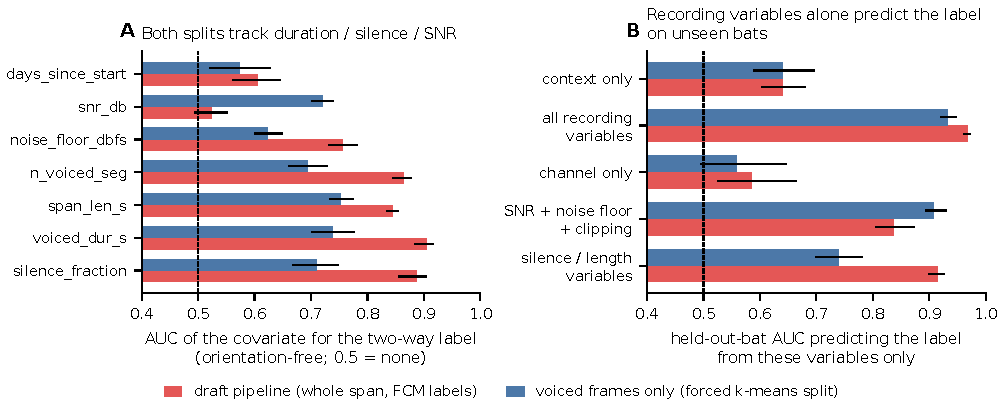
\includegraphics{fig1_v4.pdf}
\caption{(A) AUC of recording covariates for the two-way label from the original whole-span pipeline (red) and from a forced $k$-means split of voiced frames (blue). (B) Held-out-bat AUC when the label is predicted only from the listed variables. Error bars: bat-level 95\% CI.}\label{fig:conf}
\end{figure}

\subsection{Voiced frames: no balanced partition, and what the tests could detect}
With voiced frames only, FCM at $c=2$ gave FPC $=0.5000$ (the one-cluster value) for the 1,408 voiced statistics and for voiced MFCCs; whole-span MFCCs gave 0.511. Simulated single-population data with the original variance spectrum (Gaussian, heavy-tailed, skewed, and a curved one-dimensional continuum; 60 datasets each) gave FPC $\le0.503$ yet ``selected'' $c=2$ by FPC in 100\% of datasets, by silhouette in 77--100\% and by Xie--Beni in 55--63\%, while the real whole-span matrix lay outside this range (FPC 0.579, silhouette 0.220). ``All three indices select $c=2$'' is therefore uninformative: they pick the smallest $c$ tested (Supplement, Fig.~S2).

Tests that allow one cluster and resample bats agreed (Table~\ref{tab:k1}). On the voiced 1,408 statistics, prediction strength across bats was 0.66 (\ci{0.60}{0.85}), below the usual 0.8 rule and below both nulls; bootstrap Jaccard stability was 0.84 against 0.99 and 0.96; the split-sample dip statistic did not clearly exceed the nulls (0.0026 against 0.0024; permutation $p=0.16$ and $0.06$; median dip $p=0.99$, none of 40 splits below 0.05); the gap statistic chose the maximum $k$ for data and nulls alike and is not used. On the original matrix and on the whole-span features re-extracted from 15,992 files, silhouette and FPC exceeded the nulls (an excess that follows duration and SNR, Section~4.2) but prediction strength (0.70, 0.76) and the dip test did not. The silhouette and bootstrap results for voiced MFCCs and 30,000 syllable shapes were alike (Supplement Tables~S1a and S1b).

\begin{table}[!t]\centering\scriptsize
\caption{Clusterability statistics (larger = more cluster-like) against a Gaussian-copula null (cop.) and a session-mean null (ses.); mean of 50--100 null datasets. PS = prediction strength; its bat-level 95\% CI is given in the last row. The full tables for all representations are Supplement Tables~S1a and S1b.}\label{tab:k1}
\begin{tabular}{lccc|ccc|ccc}
\toprule
 & \multicolumn{3}{c|}{original matrix (true bats)} & \multicolumn{3}{c|}{voiced 1,408} & \multicolumn{3}{c}{voiced MFCC} \\
statistic & obs. & cop. & ses. & obs. & cop. & ses. & obs. & cop. & ses. \\
\midrule
FPC$(c{=}2)-0.5$ & 0.079 & 0.041 & 0.026 & 0.000 & 0.000 & 0.000 & 0.000 & 0.000 & 0.000 \\
Silhouette, $c{=}2$ & 0.221 & 0.197 & 0.181 & 0.149 & 0.128 & 0.122 & 0.159 & 0.125 & 0.108 \\
PS, $k{=}2$ & 0.704 & 0.917 & 0.712 & 0.660 & 0.955 & 0.848 & 0.789 & 0.975 & 0.875 \\
Bootstrap Jaccard, $k{=}2$ & 0.875 & 0.971 & 0.892 & 0.845 & 0.986 & 0.956 & 0.955 & 0.994 & 0.965 \\
Split-sample dip & 0.0080 & 0.0087 & 0.0074 & 0.0026 & 0.0024 & 0.0024 & 0.0021 & 0.0021 & 0.0022 \\
\midrule
PS, 95\% CI (bats) & \multicolumn{3}{c|}{\ci{0.62}{0.83}} & \multicolumn{3}{c|}{\ci{0.60}{0.85}} & \multicolumn{3}{c}{\ci{0.74}{0.93}} \\
\bottomrule
\end{tabular}
\end{table}

A negative result is informative only if the same tests would detect a discrete mixture of the same size in the same data. We therefore spiked a two-type mixture into the session-mean null of the voiced features (Fig.~\ref{fig:power}). For two equally common types, prediction strength, silhouette, bootstrap Jaccard stability and the split-sample dip statistic detected the mixture in 90--100\% of replicates at a separation of 4 standard deviations, in 48--70\% at 3 and in at most 15\% at 2. A 20\% minority was detected in 96--100\% of replicates at 6 standard deviations (47--64\% at 4), and a 5\% minority was essentially undetected up to 6 (at most 18\%) and detected only by the dip statistic at 8 (90\%). Equal-weight Gaussian mixtures become bimodal only beyond 2 standard deviations, so the battery is not unusually insensitive; but a negative result excludes well-separated common types, not overlapping, subtle or rare ones. \powersyll

\begin{figure}[!t]\centering
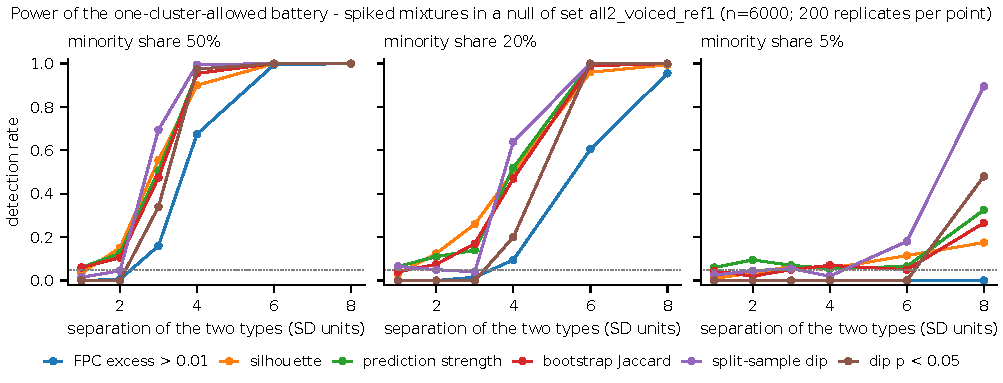
\includegraphics{fig2_v4.pdf}
\caption{Detection rate of the one-cluster-allowed battery for a two-type mixture spiked into a null with no discrete structure (voiced file-level features, 6,000 files, 200 replicates per point). The dotted line is the 5\% false-positive rate. Separation is in standard deviations along a random direction in the top ten principal components.}\label{fig:power}
\end{figure}
